\chapter{(Beyond) The Standard Model } \label{chap:SM_BSM}
The Standard Model (SM) of Particle Physics is a relativistic Quantum Field Theory (QFT) describing three out of four fundamental interactions, strong, weak and electromagnetic (EM), and the behavior of elementray particles under them.
For a long time it was attempted to merge the fourth fundamental interaction, gravity, with the SM framework, but those attempts have not been validated yet by experimental observations. Nevertheless, for our purposes, gravity does not play a significant role since the energy scales involved in the processes at a collider experiment, as the LHC, are much lower than the Planck scale, where gravitational effects become relevant.\\
What is remarkable about the SM is that it is a very well tested theory, with predictions confirmed by experimental observations with a very high precision. The discovery of the Higgs boson in 2012 at the LHC, which completed the SM framework, is a clear example of this.\\
Despite the success of the SM, there are many phenomena that are not explained by it, but are confirmed by astrophysical and cosmological observations, opening the road for Physics Beyond the Standard Model.\\
This chapter presentes a brief overview of the SM, highlighting its major features. In addition, hints for Physics Beyond it are exposed.

\section{An overview of the Standard Model} \label{sec:SM_BSM/SM}
The fundamental constituents of Universe are precisely described by the SM. They are called elementary particles, which are mathematically described as quantum fields $\psi(x)$ and their dynamics is modelled by Lagrangian densities $\mathcal{L}(\psi, \partial_{\mu}\psi)$ \cite{Peskin_QFT}. 

\begin{figure}[ht!]
    \centering
    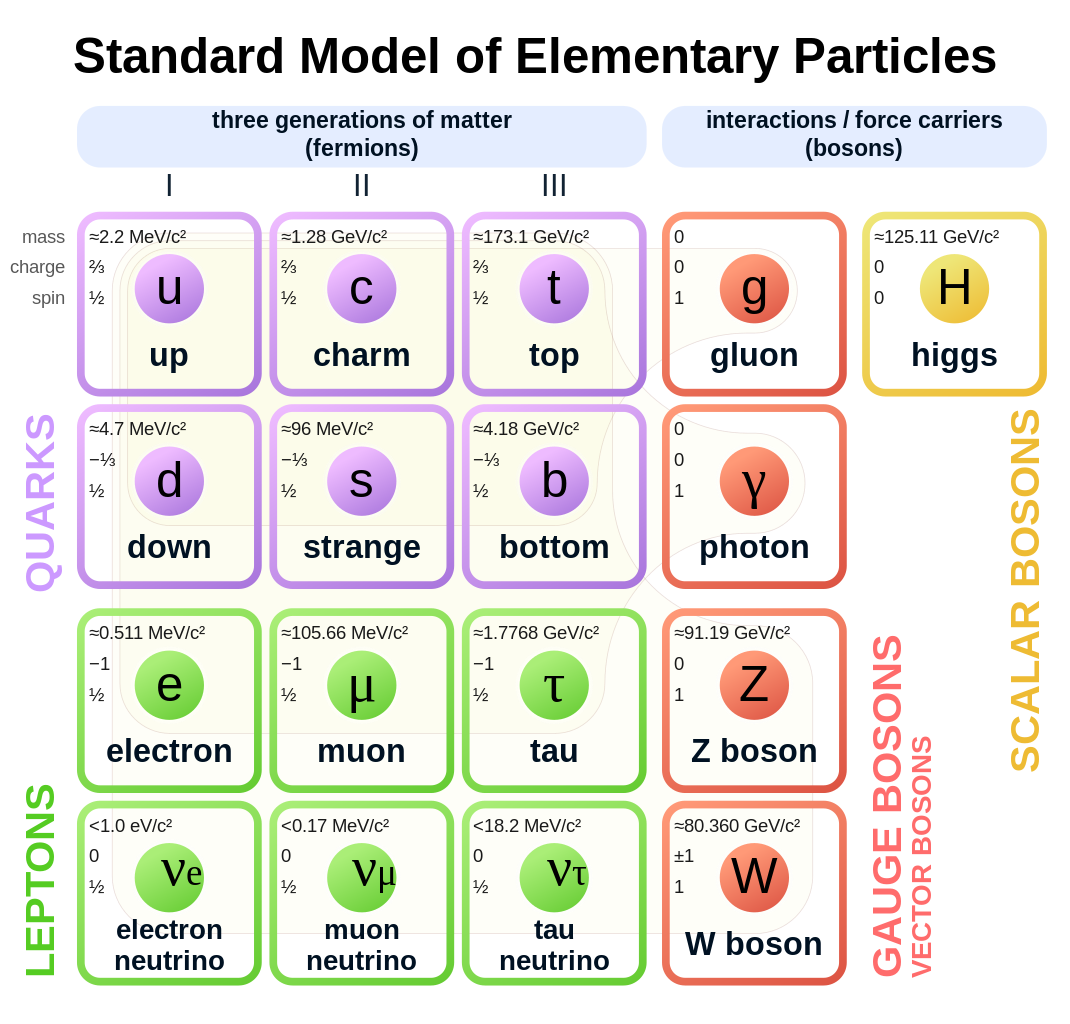
\includegraphics[width=3 in]{Images/Chap1/SM_framework.png}
    \caption{The SM framework. Figure from Ref. \cite{SM_wiki}.}
    \label{fig:SM_BSM/SM/SM_framework}
\end{figure}

\noindent Such particles can be graphically pictured as presented in Fig. \ref{fig:SM_BSM/SM/SM_framework}. 
They are divided into two fundamental classes based on their spin quantum number. The first class is composed by \textit{fermions}, which cover the first three column of Fig. \ref{fig:SM_BSM/SM/SM_framework} and are organised in three \textit{generations} of increasing proper mass; they have spin 1/2 and constitute \textit{matter}. The second class is those of \textit{bosons}, with integer spin, which \textit{mediate} fundamental interactions and generate mass.\\
Fermions are further classified into two distinct categories depending on their participation in the strong interaction. The first category is relative to \textit{quarks}. They carry \textit{colour charge} (red, green, blue), making them triplets under $SU(3)$ and therefore interact via all fundamental forces, among which the strong one.
Quarks exist in six flavors, organized into three generations of weak SU(2) doublets:
\begin{equation}\label{eq:SM_BSM/SM/quarks}
    \begin{pmatrix} u \\ d \end{pmatrix}, \quad 
    \begin{pmatrix} c \\ s \end{pmatrix}, \quad 
    \begin{pmatrix} t \\ b \end{pmatrix}
\end{equation}
Quarks carry a fractional electromagnetic charge: the \textit{up-type} ones ($u, c, t$) have a charge of $+2/3$, while the \textit{down-type} ones ($d, s, b$) carry a $-1/3$ charge.\\
The second category of fermions is associated to \textit{leptons}; they are six and similarly grouped into three generations:
\begin{equation}\label{eq:SM_BSM/SM/leptons}
    \begin{pmatrix} e^- \\ \nu_e \end{pmatrix}, \quad 
    \begin{pmatrix} \mu^- \\ \nu_\mu \end{pmatrix}, \quad 
    \begin{pmatrix} \tau^- \\ \nu_\tau \end{pmatrix}
\end{equation}
The charged leptons ($e^-, \mu^-, \tau^-$) carry an electric charge of $-1$ and interact via electromagnetic and weak forces. Neutrinos ($\nu_e, \nu_\mu, \nu_\tau$) are electrically neutral and interact exclusively via the weak force.\\
Both quarks and charged leptons, have their own anti-particles, which have the same mass of the matter components but opposite quantum numbers. Regarding neutrinos, it is still debated and to be proved whether they have a distinct anti-particles or they are Majorana fermions, being their own anti-particles.\\
The second class of particles is associated to mediatiors and mass. Spin 1 vector bosons, known as \textit{gauge bosons}, are the mediators of three of the fundamental interactions, which arise naturally from the requirement of local gauge invariance. Among those fields we find the 8 massless gluons $g$ mediating the strong interaction, the massless photon $\gamma$ is associated to electromagnetic interaction and 3 massive vector bosons, $W^\pm \text{ and } Z^0$, with masses $m_W=80.36\text{ GeV}$, $m_Z=91.19\text{ GeV}$, mediating the weak interaction.\\
In conclusion, a spin 0 scalar particle, the \textit{Higgs boson} $H$, with a mass $m_H = 125.13\text{ GeV}$, completes the particle spectrum, arising as a physical state from the spontaneous breaking of electroweak symmetry.\\

%-------------------------------------------------%
\noindent The SM is a gauge theory, meaning that the Lagrangian is invariant under local transformations of the fields. The Lagrangian density describing the SM dynamics is:

\begin{equation}\label{eq:SM_BSM/SM/SM_Lag}
\mathcal{L}_{\text{SM}} = -\frac{1}{4} F_{\mu\nu} F^{\mu\nu} - i\bar{\psi} \gamma_\mu D^\mu \psi + (D_\mu \phi)^\dagger (D^\mu \phi) - V(\phi) + \bar{\psi}_i y_{ij} \psi_j \phi + h.c.,
\end{equation}

\noindent The gauge group of the SM, under which such lagrangian is invariant, is a non-abelian symmetry group defined as:

\begin{equation}
    SU(3)_C \otimes SU(2)_L \otimes U(1)_Y
\end{equation}
\noindent where $SU(3)_C$ describes the strong interaction via Quantum Chromodynamics (QCD) with subscript \textit{C} standing for colour, and $SU(2)_L \otimes U(1)_Y$ represents the unified electroweak (EW) interaction, with \textit{L} associated to the left component of fermions and \textit{Y} to hypercharge.\\
The terms of the equation \ref{eq:SM_BSM/SM/SM_Lag} above are presented in detail in the following sections.

%-------------------------------------------------------------------------------
\subsection{Quantum Electrodynamics}\label{subsec:SM_BSM/SM/QED}
The first and simplest gauge theory within the SM framework is Quantum Electrodynamics (QED). It describes the electromagnetic interactions between a charged massive fermion, with mass \textit{m} and represented by a field $\psi(x)$, and the photon, the massless gauge boson represented by the vector field $A_\mu$.
Using the Lagrangian formalism \cite{Feynman_QFT}, QED is constructed starting from the free Dirac Lagrangian for a massive fermion \cite{pich_QED_EW}:

\begin{equation}\label{eq:SM_BSM/QED/Dirac_L}
    \mathcal{L}_\text{Dirac} = \bar{\psi} (i\gamma^\mu \partial_\mu - m) \psi
\end{equation}

\noindent In the equation above, $\bar{\psi} = \psi^\dagger \gamma^0$ is the Dirac adjoint of the field $\psi$ and $\gamma^\mu$ are the Dirac matrices derived from Pauli matrices $\sigma_i$ ($i$ =1,2,3 and $\mu$=0,1,2,3): 

\begin{equation}\label{eq:SM_BSM/QED/PauliMatrix}
\gamma^0 = \begin{pmatrix} 0 & \mathbb{I} \\ \mathbb{I} & 0 \end{pmatrix}, \qquad
\gamma^i = \begin{pmatrix} 0 & \sigma_i \\ -\sigma_i & 0 \end{pmatrix}
\end{equation}

\noindent The Dirac Lagrangian \ref{eq:SM_BSM/QED/Dirac_L} is invariant under a global $U(1)$ phase transformation $\psi(x) \to e^{i e \alpha} \psi(x)$, with $e$ the electric charge of the fermion and $\alpha$ a constant phase.
Such invariance is not preserved under a local $U(1)$ phase transformation $\psi(x) \to e^{i e \alpha(x)} \psi(x)$, where $\alpha(x)$ is a space-time dependent phase. In order to preserve the invariance, the partial derivative $\partial_\mu$ is replaced by the covariant derivative $D_\mu$:

\begin{equation}\label{eq:SM_BSM/QED/cov_der}
    D_\mu = \partial_\mu + i e A_\mu(x)
\end{equation}
where $A_\mu(x)$ is a vector gauge field representing the photon field, which transforms as $A_\mu(x) \to A_\mu(x) - \partial_\mu \alpha(x)$. Including the gauge-invariant kinetic term to take into account for the new field $A_\mu$, we derive the full QED Lagrangian:

\begin{equation}\label{eq:SM_BSM/QED/QED_L}
    \mathcal{L}_\text{QED} = \bar{\psi} (i\gamma^\mu D_\mu - m) \psi - \frac{1}{4} F_{\mu\nu} F^{\mu\nu}
\end{equation}
where $F_{\mu\nu} = \partial_\mu A_\nu - \partial_\nu A_\mu$ is the electromagnetic field strength tensor. The interaction term $-e \bar{\psi} \gamma^\mu \psi A_\mu$ rules the coupling of charged fermions to photons with a strength proportional to the electric charge $e$.


\subsection{Quantum Chromodynamics}\label{subsec:SM_BSM/SM/QCD}
\subsection{Electroweak model}\label{subsec:SM_BSM/SM/EW}

\section{Hints of Physics Beyond the Standard Model}\label{sec:SM_BSM/BSM}


/////////////////////////////////////////// \\

%-------------------------------------------------------------------------------


%-------------------------------------------------------------------------------
\subsection{Quantum Chromodynamics}
\label{subsec:qcd}

Quantum Chromodynamics (QCD) is the non-Abelian gauge theory describing the strong force acting between color-charged quarks and gluons. QCD is based on the local $SU(3)_C$ gauge symmetry, where $C$ represents the triplet color degree of freedom (red, green, blue). The Lagrangian for $N_f$ quark flavors is given by:
\begin{equation}
    \mathcal{L}_\text{QCD} = \sum_{f} \bar{q}_f^a \left( i \gamma^\mu (D_\mu)_{ab} - m_f \delta_{ab} \right) q_f^b - \frac{1}{4} G_{\mu\nu}^A G^{A, \mu\nu}
\end{equation}
where $q_f^a$ represents a quark field of flavor $f$ and color index $a \in \{1, 2, 3\}$. The gauge-covariant derivative is defined as:
\begin{equation}
    (D_\mu)_{ab} = \partial_\mu \delta_{ab} - i g_s T^A_{ab} A_\mu^A
\end{equation}
where $g_s$ is the strong coupling constant, $A_\mu^A$ ($A = 1, \dots, 8$) are the eight gluon vector fields, and $T^A = \frac{1}{2} \lambda^A$ are the $SU(3)$ generators expressed via the Gell-Mann matrices satisfying $[T^A, T^B] = i f^{ABC} T^C$.

The non-Abelian structure gives rise to the field strength tensor:
\begin{equation}
    G_{\mu\nu}^A = \partial_\mu A_\nu^A - \partial_\nu A_\mu^A + g_s f^{ABC} A_\mu^B A_\nu^C
\end{equation}
The presence of the non-linear structure constant term $f^{ABC}$ introduces triple and quadruple gluon self-interactions. This characteristic yields two defining physical properties of QCD:
\begin{enumerate}
    \item \textbf{Asymptotic Freedom:} At high energy scales (short distances), the running coupling constant $\alpha_s(Q^2) = \frac{g_s^2}{4\pi}$ decreases logarithmically, enabling accurate calculations via perturbative QCD (pQCD).
    \item \textbf{Color Confinement:} At low energy scales (long distances), $\alpha_s(Q^2)$ grows large. Colored particles cannot exist as isolated free states; they undergo fragmentation and hadronization, producing collimated sprays of energetic, neutral hadrons known as \textbf{jets}.
\end{enumerate}

%-------------------------------------------------------------------------------
\subsection{Electroweak Model}
\label{subsec:electroweak}

The unification of electromagnetic and weak interactions is realized through the Glashow-Weinberg-Salam (GWS) model, structured around the local gauge symmetry group $SU(2)_L \times U(1)_Y$. The left-handed fermion components transform as doublets under weak isospin $T$, whereas right-handed components transform as singlets:
\begin{equation}
    \Psi_L = \begin{pmatrix} \nu_{L} \\ e_L^- \end{pmatrix} \quad (T = 1/2, T_3 = \pm 1/2), \qquad e_R^- \quad (T = 0, T_3 = 0)
\end{equation}
Electric charge $Q$, weak isospin $T_3$, and weak hypercharge $Y$ are unified by the Gell-Mann-Nishijima relation:
\begin{equation}
    Q = T_3 + \frac{Y}{2}
\end{equation}

The gauge-covariant derivative introducing three $W_\mu^i$ ($i=1,2,3$) bosons for $SU(2)_L$ and one $B_\mu$ boson for $U(1)_Y$ is written as:
\begin{equation}
    D_\mu = \partial_\mu - i g T^i W_\mu^i - i g' \frac{Y}{2} B_\mu
\end{equation}

Spontaneous Symmetry Breaking (The Higgs Mechanism)
Unbroken $SU(2)_L \times U(1)_Y$ symmetry forbids mass terms for gauge bosons and fermions, as explicit mass terms violate local gauge invariance. Mass generation is accommodated via the Brout-Englert-Higgs mechanism by introducing a complex scalar doublet field $\Phi$:
\begin{equation}
    \Phi = \frac{1}{\sqrt{2}} \begin{pmatrix} \phi^+ \\ \phi^0 \end{pmatrix}, \quad \mathcal{V}(\Phi) = \mu^2 \Phi^\dagger \Phi + \lambda (\Phi^\dagger \Phi)^2 \quad (\mu^2 < 0, \lambda > 0)
\end{equation}
The scalar field acquires a non-zero vacuum expectation value (VEV) $v = \sqrt{-\mu^2/\lambda} \approx 246\text{ GeV}$, spontaneously breaking the symmetry:
\begin{equation}
    SU(2)_L \times U(1)_Y \xrightarrow{\text{SSB}} U(1)_\text{EM}
\end{equation}
Expanding $\Phi$ around its minimum in the unitary gauge transforms three degrees of freedom into longitudinal polarization states for the gauge physical bosons $W^\pm$ and $Z^0$:
\begin{equation}
    W_\mu^\pm = \frac{1}{\sqrt{2}}(W_\mu^1 \mp i W_\mu^2), \quad 
    \begin{pmatrix} Z_\mu \\ A_\mu \end{pmatrix} = \begin{pmatrix} \cos\theta_W & -\sin\theta_W \\ \sin\theta_W & \cos\theta_W \end{pmatrix} \begin{pmatrix} W_\mu^3 \\ B_\mu \end{pmatrix}
\end{equation}
where $\theta_W = \arctan(g'/g)$ is the weak mixing angle. The photon field $A_\mu$ remains massless, while gauge bosons acquire masses $m_W = \frac{1}{2} g v$ and $m_Z = \frac{1}{2} v \sqrt{g^2 + g'^2}$. Fermions acquire mass through gauge-invariant Yukawa couplings:
\begin{equation}
    \mathcal{L}_\text{Yukawa} = -y_f \bar{\Psi}_L \Phi f_R + \text{h.c.} \quad \implies \quad m_f = \frac{y_f v}{\sqrt{2}}
\end{equation}

%-------------------------------------------------------------------------------
\section{Hints of Physics Beyond the Standard Model}
\label{sec:bsm}

Despite the extraordinary predictive precision of the Standard Model—culminating in the discovery of the Higgs boson at the LHC in 2012~\cite{ATLAS:2012, CMS:2012}—it cannot be regarded as a complete theory of fundamental interactions. Unresolved theoretical open issues and physical phenomena observed in nature mandate the existence of Physics Beyond the Standard Model (BSM)~\cite{Garrett:2011}:

\begin{itemize}
    \item \textbf{Dark Matter:} Astrophysical and cosmological observations (galaxy rotation curves, gravitational lensing, cosmic microwave background) firmly establish that non-baryonic \textit{Dark Matter} comprises $\approx 26.8\%$ of the energy density of the Universe~\cite{Garrett:2011}. The SM offers no suitable stable, cold, weakly-interacting candidate particle~\cite{Garrett:2011}.
    
    \item \textbf{Neutrino Masses:} Oscillations observed in solar, atmospheric, and reactor neutrinos demonstrate that neutrinos possess non-zero masses, contrasting the strict masslessness assumed in the minimal SM structure.
    
    \item \textbf{Baryon Asymmetry:} The observable universe consists almost entirely of matter rather than antimatter~\cite{Garrett:2011}. The magnitude of $CP$ violation provided by the SM CKM matrix is insufficient to account for the observed cosmic matter-antimatter asymmetry~\cite{Garrett:2011}.
    
    \item \textbf{The Hierarchy Problem:} Quantum loop corrections to the scalar Higgs boson mass quadratic divergences yield corrections proportional to the Planck scale ($\Lambda_{\text{Planck}} \approx 10^{19}\text{ GeV}$). Maintaining $m_H \approx 125\text{ GeV}$ requires extreme, fine-tuned cancellations without a protective symmetry (such as Supersymmetry).
    
    \item \textbf{Quantum Gravity:} The Standard Model does not incorporate gravitational interactions. A quantum formulation of gravity compatible with General Relativity remains omitted at high energy scales.
\end{itemize}

These limitations motivate the search for new BSM resonance states and heavy new physics at collider experiments like the Large Hadron Collider (LHC)[cite: 9].